\documentclass{article}
\usepackage{graphicx}
\usepackage{ctex}
\usepackage{listings}


\title{基于K-Means算法的图像分割}
\author{王铭嵩}
\date{\today}

\begin{document}
\maketitle
\section{K-Means算法概述}
\subsection{原理}
K-Means算法是一种无监督分类算法,该算法的任务是将无标签数据集聚类成k个簇,利用贪心策略求得近似解。
具体步骤为:
\begin{enumerate}
    \item 在样本集中随机选取$k$个样本作为初始各簇中心点$\mu_{i}$。
    \item 计算所有样本点与各个簇中心之间的距离,并将其划入最近的簇中。
    \item 根据簇中已有的样本点,重新计算簇中心$\mu_{i}=\frac{1}{|C_{i}|}\sum_{x\in{C{i}}}x$
    \item 重复2,3.
\end{enumerate}
\subsection{优化}
K-Means++优化了各簇中心点的选取:
\begin{enumerate}
    \item 随机选取一个样本点作为第一个簇中心$\mu_1$,
    \item 计算剩余样本点与所有簇中心的最短距离,$D(x^{(i)})=min[dist(x^{(i)},C_j)|j=1,2,...,n]$,某样本点被选为下一个簇中心的概率为$\frac{D(x^{(i)})^2}{\Sigma D(x^{(j)})^2}$,
    \item 重复2,直到选出k个簇中心。
\end{enumerate}
\section{实验过程}
\subsection{图片输入}
输入图片:\\

\includegraphics[width=1.0\textwidth]{../python/crane.jpg}\\
已将原始图片的宽高等比缩放之原来的25\%。

\subsection{代码实现}
\lstset{
    language=python,
    frame=shadowbox,
    breaklines=true
}
首先利用cv2库读入图片,并利用numpy将图片转化为二维数组,其中每一行代表一个像素,包含RGB三个列的值。
\begin{lstlisting}
    # read the image
    image = cv2.imread('crane.jpg')
    
    # break the image into 2D array
    pixels = image.reshape(-1, 3)
\end{lstlisting}
然后创建KMeans对象,并利用fit方法和predict方法得到聚类后的结果。
\begin{lstlisting}
    kmeans = KMeans(n_clusters=cluster_cnt)
    kmeans.fit(pixels)
    labels = kmeans.predict(pixels)
\end{lstlisting}
最后将聚类后的结果转化为图片,并保存和展示。
\begin{lstlisting}
    # reconstructed segmented image
    segmented_image = labels.reshape(image.shape[0], image.shape[1])

    segments=[]

    for i in range(cluster_cnt):
        segments.append(np.copy(image))
        segments[i][segmented_image != i] = 0

    # display and save the segmented images
    for i in range(cluster_cnt):
        cv2.imshow('Segment '+str(i), segments[i])
        cv2.imwrite('Segment '+str(i)+'.png', segments[i])
    cv2.waitKey(0)
    cv2.destroyAllWindows()
\end{lstlisting}
\subsection{结果展示}
聚类结果:
\subsubsection{clusters=2, iterations=300}
使用KMeans.py实现。\\

\includegraphics[width=0.5\textwidth]{src/it=300_0.png}
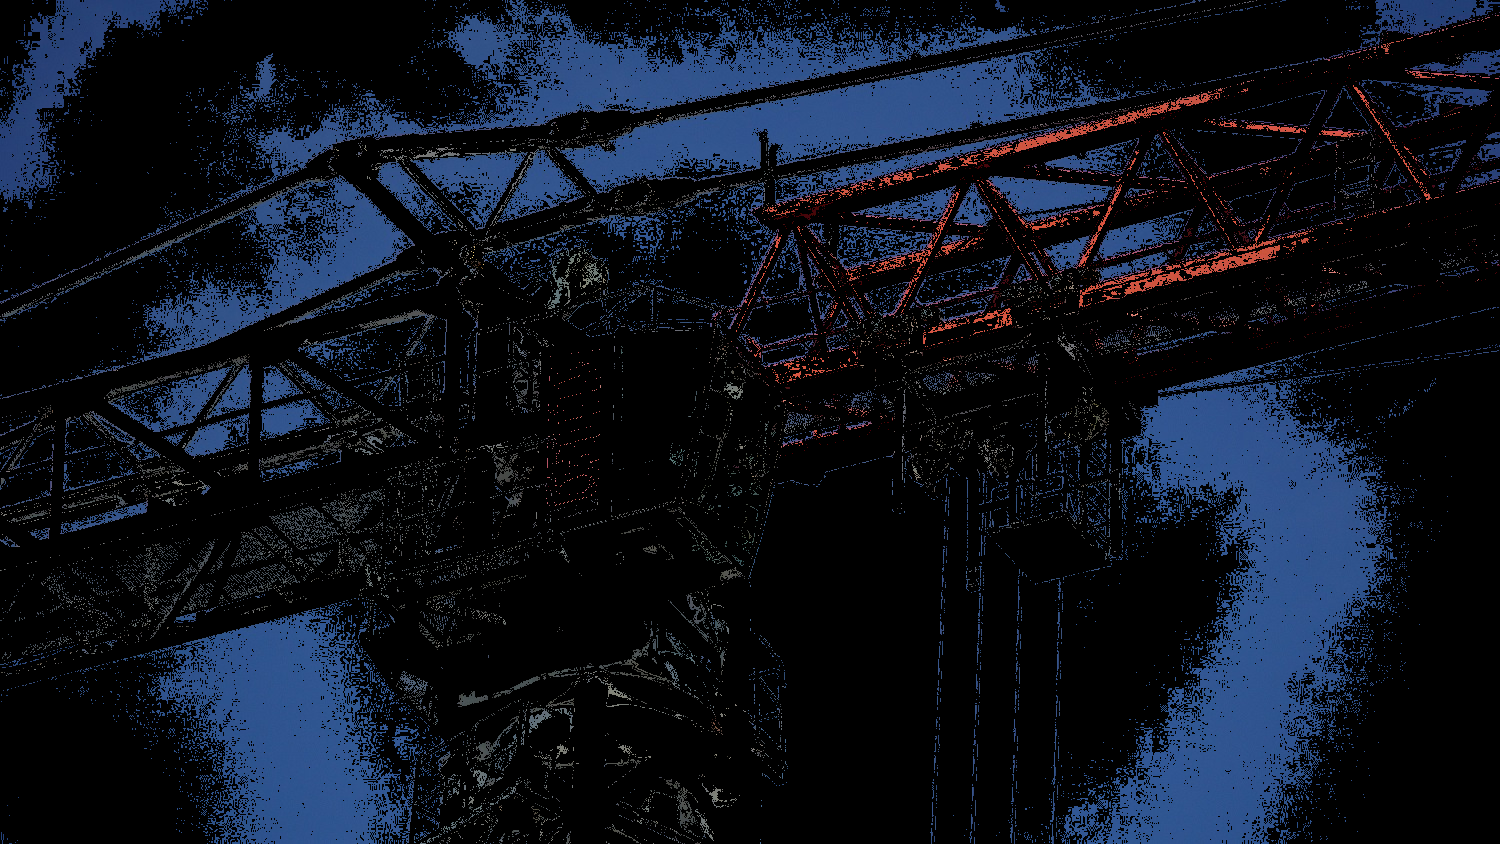
\includegraphics[width=0.5\textwidth]{src/it=300_1.png}\\
\subsubsection{clusters=2, iterations=3000}
使用KMeans.py实现。\\

\includegraphics[width=0.5\textwidth]{src/it=3000_0.png}
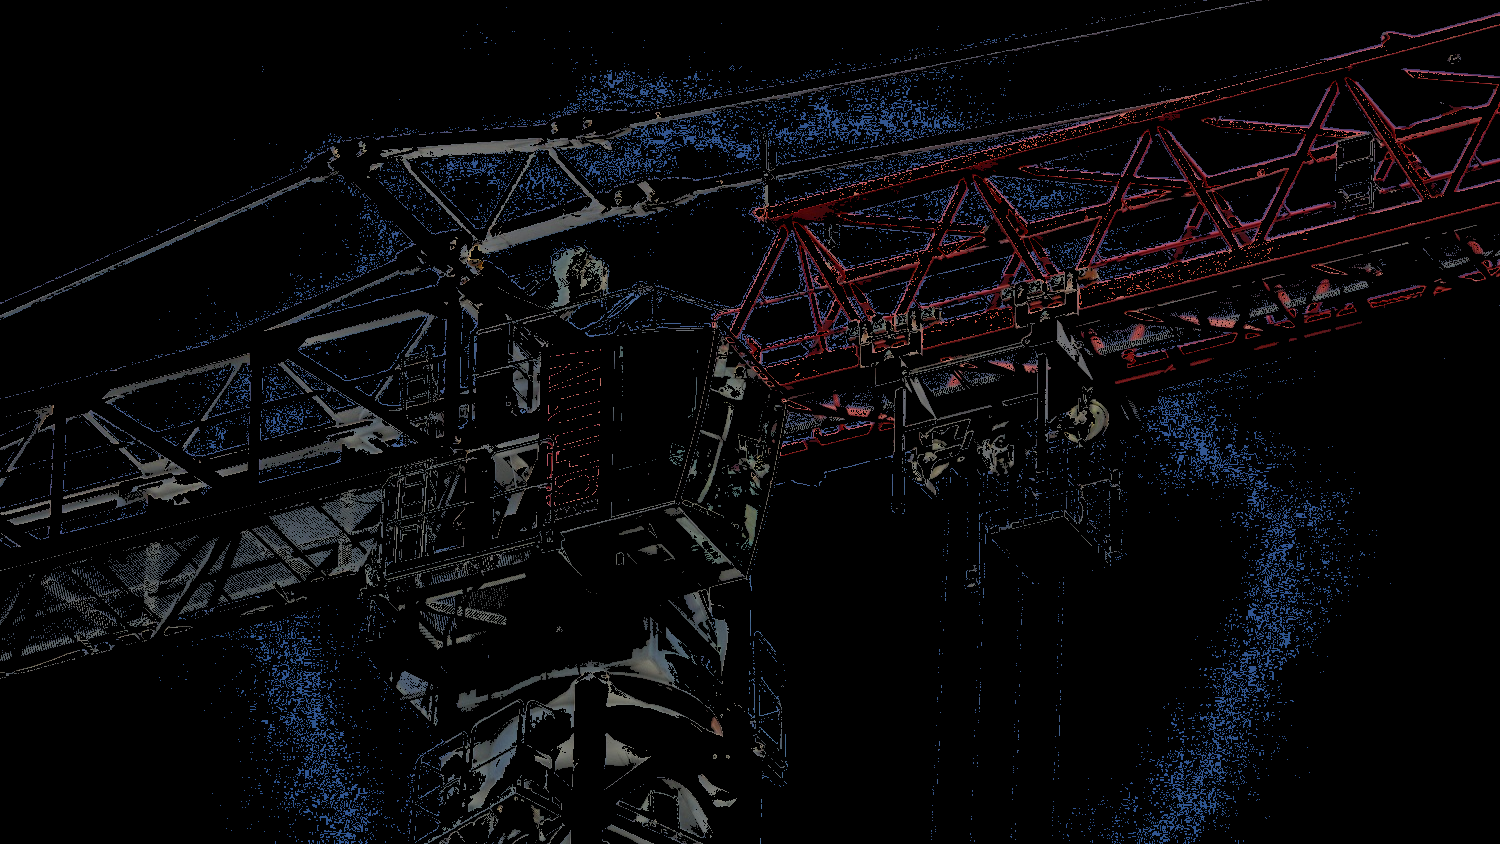
\includegraphics[width=0.5\textwidth]{src/it=3000_1.png}\\
\subsubsection{clusters=3, iterations=default}
使用sklearn库实现。\\
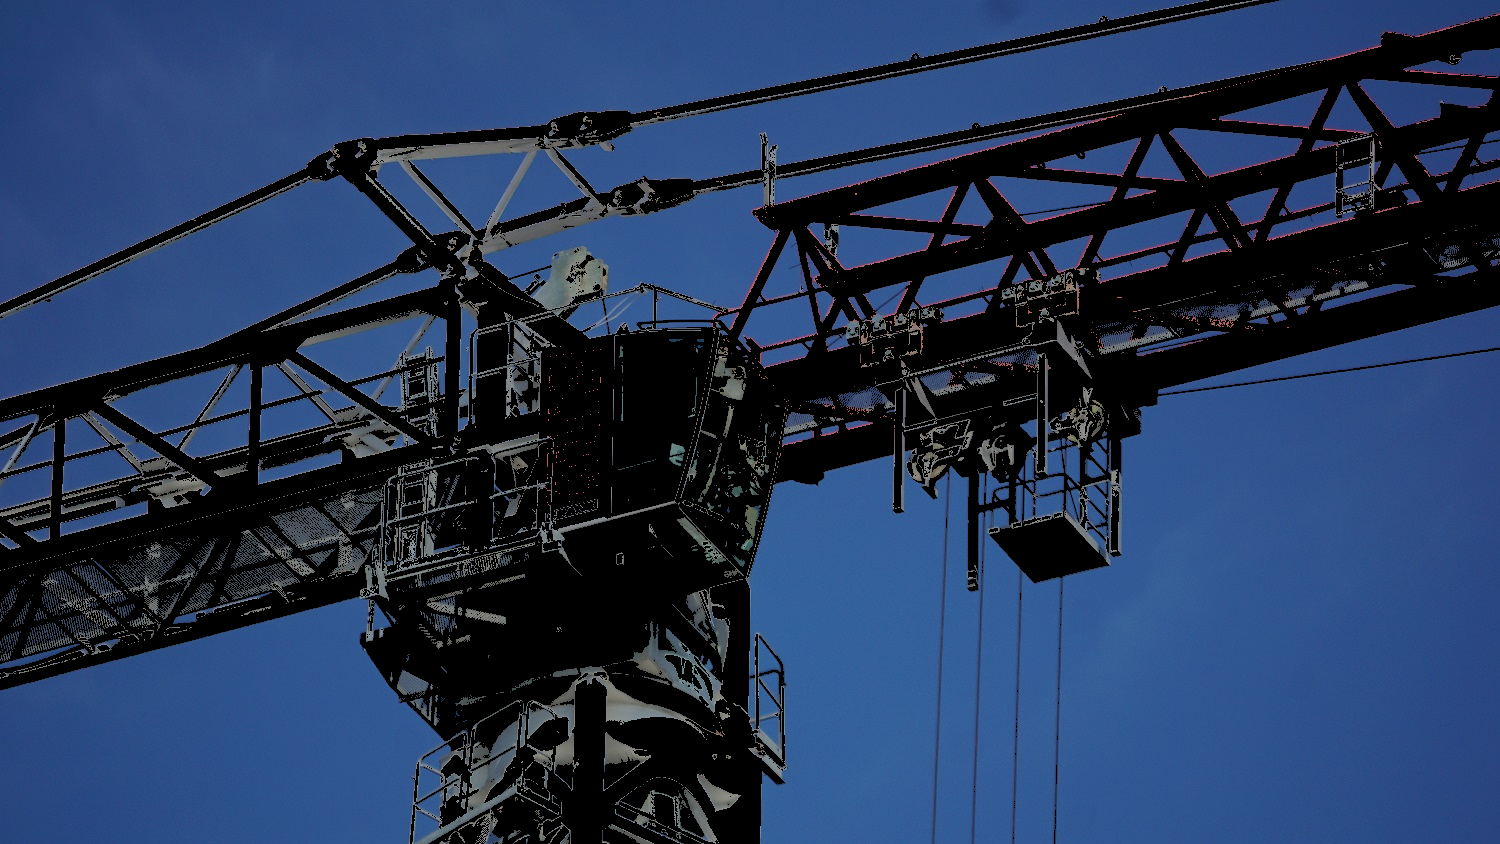
\includegraphics[width=0.33\textwidth]{src/sklearn_0.png}
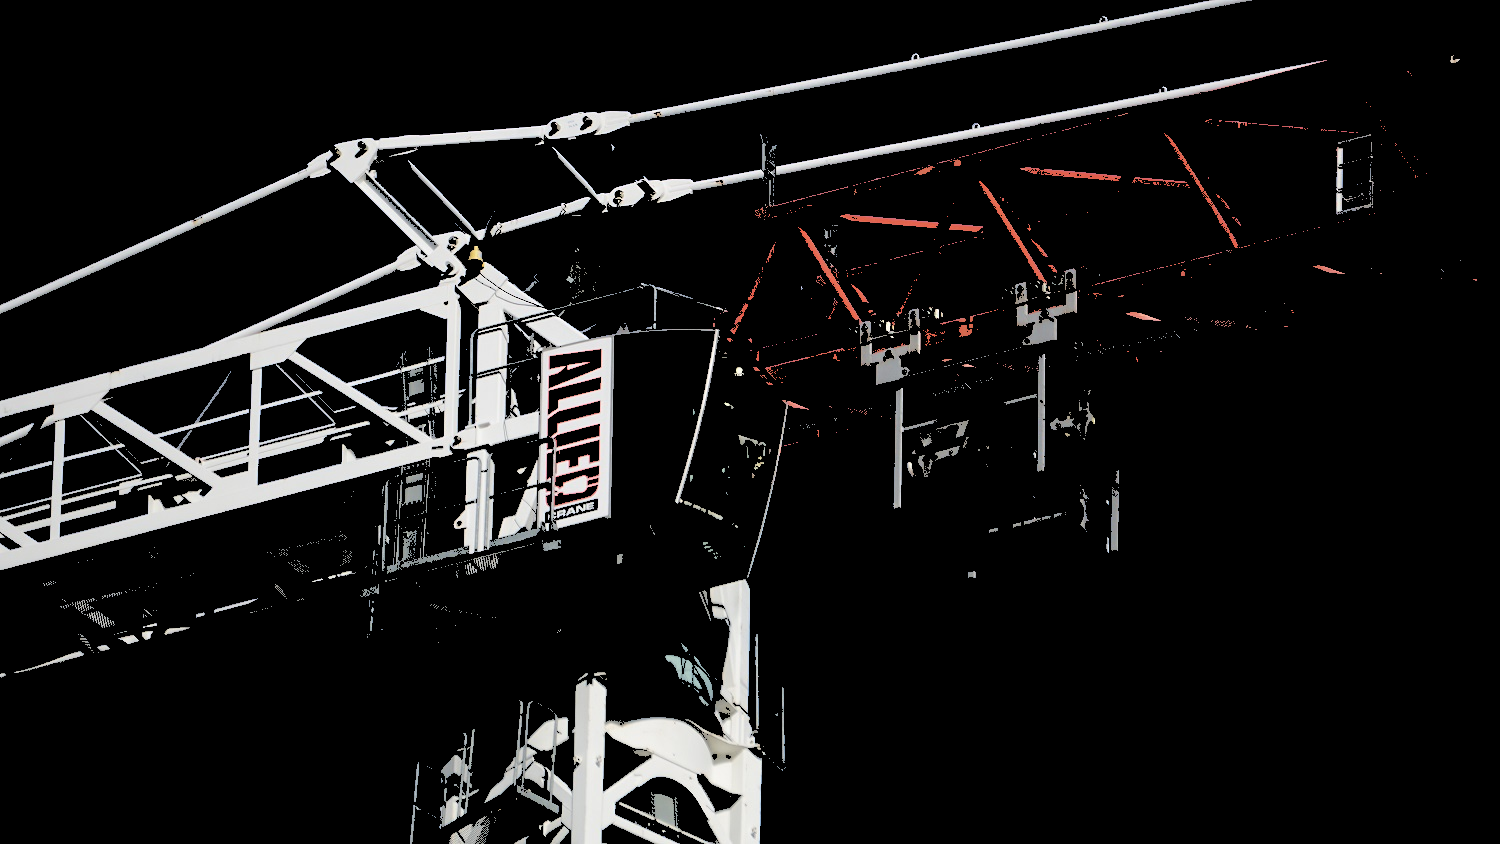
\includegraphics[width=0.33\textwidth]{src/sklearn_1.png}
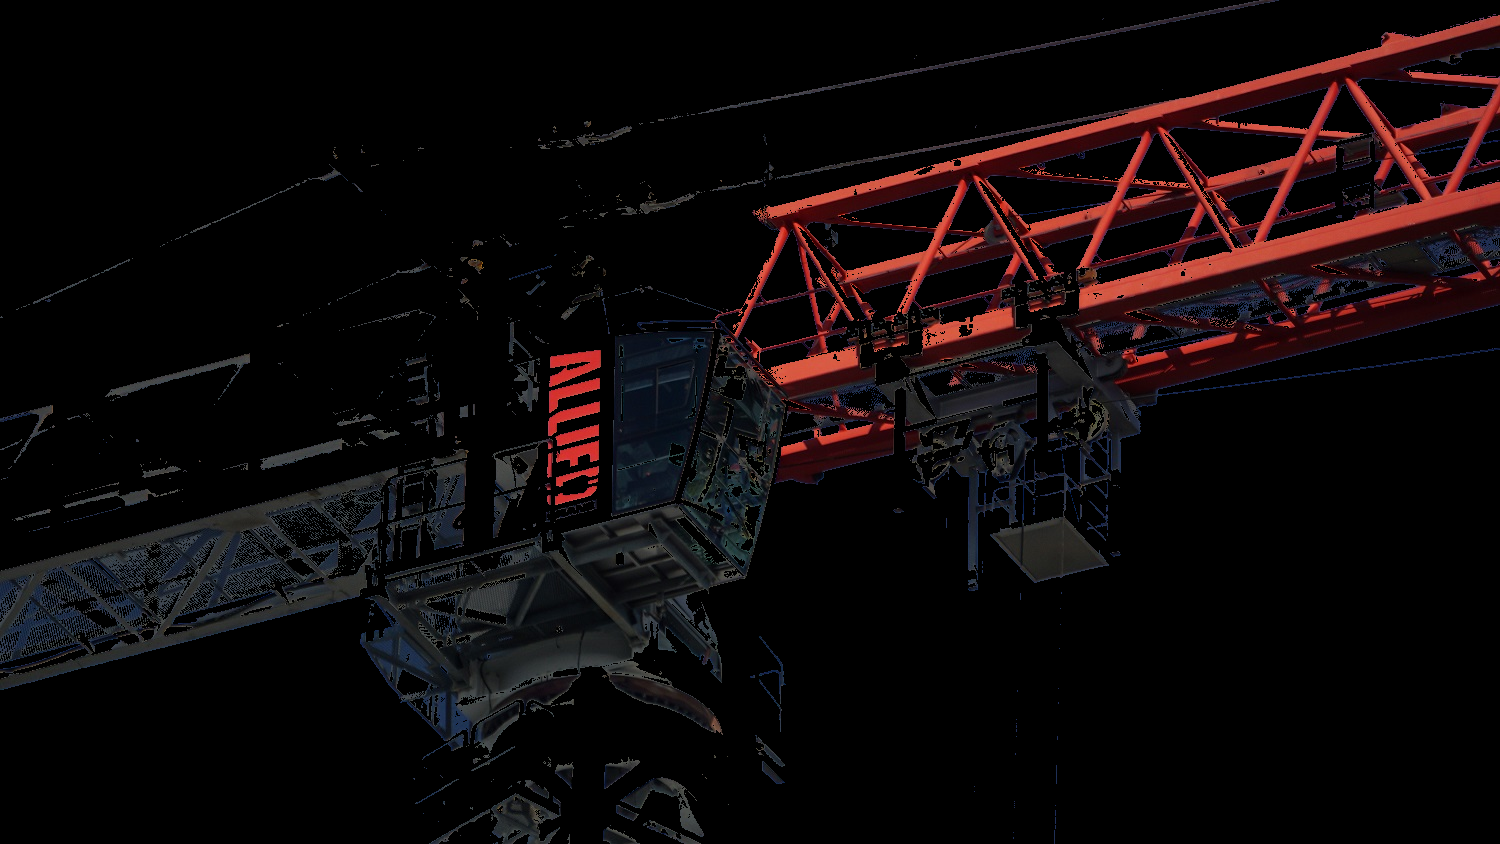
\includegraphics[width=0.33\textwidth]{src/sklearn_2.png}\\
\subsubsection{问题}
sklearn库中的KMeans默认采用Lloyd算法,距离计算采用欧氏距离;而KMeans.py中的KMeans调用向量取模函数,在距离算法上应该与其相同,但结果却与sklearn库大相径庭。可能是在选点和迭代条件上有约束?
\end{document}